\documentclass[opre,copyedit]{informs1}
\usepackage{amsmath}
\usepackage{amssymb}
\usepackage{latexsym}
\usepackage{CJK}
\usepackage{longtable}
\usepackage{supertabular}
\usepackage{secdot,lscape}
\usepackage{url}
\usepackage{xcolor}
\usepackage{graphicx,graphics,epsfig}
\usepackage{float}

%\usepackage{graphics,color,graphicx,epsfig,amsmath,amssymb,amsthm,amsopn}

\long\def\ajm#1{{\color{black}#1}}
\newcommand{\ignore}[1]{}
\newcommand{\E}{\mbox{\sf E}}
\newcommand{\tabincell}[2]{\begin{tabular}{@{}#1@{}}#2\end{tabular}}

\newenvironment{proof}{}{\hfill\rule{2mm}{2mm}}

\theoremstyle{TH}
%\theoremstyle{definition}
\newtheorem{thm}{Theorem}
\newtheorem{lem}[thm]{Lemma}
\newtheorem{prop}[thm]{Proposition}
\newtheorem{cor}[thm]{Corollary}
\newtheorem{supportingLemma}{Lemma}[section]
\newtheorem{supportingProp}{Proposition}[section]
\newtheorem{asm}[thm]{Assumption}
\newtheorem{mydef}{Definition}

%%% OPRE uses endnotes
\usepackage{endnotes}
\let\footnote=\endnote
\let\enotesize=\normalsize
\def\notesname{Endnotes}%
\def\makeenmark{\hbox to1.275em{\theenmark.\enskip\hss}}
\def\enoteformat{\rightskip0pt\leftskip0pt\parindent=1.275em
\leavevmode\llap{\makeenmark}}

% Natbib setup for author-year style
\usepackage{natbib}
 \bibpunct[, ]{(}{)}{,}{a}{}{,}%
 \def\bibfont{\small}%
 \def\bibsep{\smallskipamount}%
 \def\bibhang{24pt}%
 \def\newblock{\ }%
 \def\BIBand{and}%

%% Setup of theorem styles. Outcomment only one.
%% Preferred default is the first option.
\TheoremsNumberedThrough     % Preferred (Theorem 1, Lemma 1, Theorem 2)
%\TheoremsNumberedByChapter  % (Theorem 1.1, Lema 1.1, Theorem 1.2)

%% Setup of the equation numbering system. Outcomment only one.
%% Preferred default is the first option.
\EquationsNumberedThrough    % Default: (1), (2), ...
%\EquationsNumberedBySection % (1.1), (1.2), ...
\newcommand{\beq}[1] {\begin{equation} \label{#1}}
\newcommand{\eeq}{\end{equation}}
\newcommand{\bed}{\begin{displaymath}}
\newcommand{\eed}{\end{displaymath}}
\newcommand{\bedd}{\bed\begin{array}{l}}
\newcommand{\eedd}{\end{array}\eed}
\newcommand{\nd}{\noindent}

\newcommand{\bea}{\begin{eqnarray}}
\newcommand{\eea}{\end{eqnarray}}
\newcommand{\bean}{\begin{eqnarray*}}
\newcommand{\eean}{\end{eqnarray*}}
\newcommand{\dF}{\dot{F}}
\newcommand{\dlm}{\dot{\lambda}}

\newcommand{\lm}{\lambda}
\newcommand{\nn}{\nonumber\\}
\newcommand{\ra}{\rightarrow}
\newcommand{\vep}{\varepsilon}
\newcommand{\bF}{\overline{F}}
\newcommand{\bp}{\overline{p}}
\newcommand{\blm}{\overline{\lm}}
\newcommand{\lra}{\longrightarrow}
\newcommand{\bdd}{\hspace*{-0.08in}{\bf.}\hspace*{0.05in}}

\def\disp{\displaystyle}
% In the reviewing and copyediting stage enter the manuscript number.
\MANUSCRIPTNO{} % When the article is logged in and DOI assigned to it,
                % this manuscript number is no longer necessary

\setlength{\textwidth} {6.5in}
\setlength{\textheight} {9.1in}
\setlength{\oddsidemargin} {0.0in}
\setlength{\topmargin} {0.0in}

%\documentstyle[12pt]{article}
%\setlength{\oddsidemargin}{-0.3in}
%\setlength{\evensidemargin}{0in}
%\setlength{\textheight}{9.5in}
%\setlength{\textwidth}{6.8in}
%\setlength{\topmargin}{-0.5in}
%
%\newtheorem{thm}{Theorem}
%\newtheorem{prop}{Proposition}
%\newtheorem{lem}{Lemma}
%\newtheorem{rem}{Remark}
%\newtheorem{cor}{Corollary}
%\newtheorem{defn}{Definition}
%\newtheorem{exm}{Example}
%\newtheorem{asm}{Assumption}

%\newcommand{\thmref}[1]{Theorem~{\rm \ref{#1}}}
%\newcommand{\lemref}[1]{Lemma~{\rm \ref{#1}}}
%\newcommand{\corref}[1]{Corollary~{\rm \ref{#1}}}
%\newcommand{\propref}[1]{Proposition~{\rm \ref{#1}}}
%\newcommand{\defref}[1]{Definition~{\rm \ref{#1}}}
%\newcommand{\remref}[1]{Remark~{\rm \ref{#1}}}
%\newcommand{\exmref}[1]{Example~{\rm \ref{#1}}}
%\newcommand{\asmref}[1]{Assumption~{\rm \ref{#1}}}

%\renewcommand{\theequation}{\thesection.\arabic{equation}}
%\newcommand{\mysection}[1]{\section{#1}\setcounter{equation}{0}}


\begin{document}

\TITLE{Loss Given Default Modeling for Online Microloan \footnote{Corresponding author: Telephone: 86-21-65901032, Fax: 86-21-65901099,  Email: luo.sirong@mail.shufe.edu.cn}}

%\ARTICLEAUTHORS{
%\AUTHOR{Sirong Luo \hspace{1.5cm} Xiao Kong \hspace{1.5cm} Tingting Nie }
%\AFF{School of Statistics and Management, Shanghai University of Finance and Economics \\ 777 Guoding Road, Shanghai 200433, China \\
%\EMAIL{Luo.Sirong@mail.shufe.edu.cn} \URL{}}
%}

%\date{}
%\HISTORY{Nov, 16, 2013}

\ABSTRACT{In this project, we study the LGD modeling for online microloan using a real online P2P lending dataset. We first analyze the characteristics of LGD for online microloans, then, we explore different statistical models for LGD modeling including both parametric model and semi-parametric model. For zero RRs and non-zeros, we build two discriminant models, while two continuous models for RRs fell in $(0,1)$. Finally, we assess the prediction performance of these models on a validation sample.}

\KEYWORDS{Peer to Peer Lending, Credit Risk Scoring, Loss Given Default, Quantile Regression}

\maketitle

\vspace{-0.3in}
\section{Introduction}
Over the past decade, online microloan market has rapidly grown into a popular business model
across the world. It leverages online platforms to connect individual borrowers with individual
lenders (i.e., investors), and it has proven to be a very viable business model. For example, the two largest peer-to-peer (P2P) lending platforms, Prosper and Lending Club founded in 2005 and 2006 respectively, have originated over \$6 Billion in loans to date. In the P2P platform, to start the loan process, a borrower posts a loan-request listing on an online P2P lending platform, and the prospective investors (i.e., lenders) who are interested in the listing start bidding on portions of the loan - the contracted interest rate of a funded listing is either determined by the auction or by the platform. For a funded listing, the borrower is obligated to pay off the principal and the accumulated interests when the loan matures. Ideally, P2P lending model produces a win-win situation for both parties. For a paid-off loan, the investors are better off having gained more interests than simply parking her money in banks saving accounts. From the standpoint of the borrower, he is also better off having obtained the credit that he would have difficulty obtaining from the traditional financial intermediaries, such as banks and credit cards. However, it is often to
see that some borrowers eventually default on their loans, leaving the lenders suffering substantial financial losses. According to Renton (2014), the default rate of the loans on the P2P lending platforms is usually relative high, and in some cases could reach as high as 30\%. Therefore, the loss estimation is critical for both platform and investors. Platform need accurate loss estimation to provide credit rating and set the borrow rate. For investors, the improved estimation of loss can help them make better investment decisions. To estimate the loss, we need predict the default risk and the loss given default (LGD). In this project, we will focus on the statistical estimation of LGD.
Specifically, we will first investigate the characteristics of loss given default for online microloans, then, we will explore different statistical tools to build better prediction models for LGD.

\section{Literature Review}\label{sec:LR}

Online P2P lending has become more and more popular recently. Some researchers even think it has a chance to disintermediate the finance market. As a convenient way for personal borrowing and lending, it bears high risk. We tried some loss modeling methods as a benchmark to investigate the relationship between default and given private and environment variables so that we can use them to predict the potential loss of an online loan. After that we hire the quantile regression modeling method as a way to measure the heterogeneity in some variables. It turns out that the quantile method gives improved results.

\subsection{Online P2P Lending}\label{sec:P2P}

The two largest peer-to-peer (P2P) lending platforms, Prosper and Lending Club founded in 2005 and 2006 respectively, have originated over \$6 Billion in loans to date. There's two main parts has been given most attention to: whether the electronic credit marketplace will lead to disintermediation by replacing financial institutions as the traditional intermediary, and to what extent it relies on social networks. \citet{Hulme2006} studied one of the top 10 sites of P2P lending-Zopa and point out that social lending schemes as a newly emerging type of financial relationship will contribute to the disintermediation of financial markets by rivaling traditional financial services and challenging the traditional banking model. \citet{Herzenstein2008} paid attention to compare the impact of demographic attributes, borrowers�� financial strength and their effort indicator on the likelihood of funding success and found the first aspect less effective. \citet{Collier2010} focused on the community reputation systems while \citet{Duarte2012} studied the relationship between the appearance and trustworthiness of borrowers, and how it impacts the probability of funding in online P2P lending. \citet{BellottiC2012} tried classical parametric and nonparametric methods to investigate the credit cards data sets, and they found the inclusion of macroeconomic variables (MV) is important. \citet{Ghasemkhani2013} provided a research on the impact of reputation and friendship networks on electronic credit market outcomes and empirically show that using such non-credit-related information can help mitigate the concern that the disintermediation of the financial market driven by information technology might cause a loss of soft information and suffer from the adverse selection problem. \citet{Leow2014} also did some work about MVs in UK retail lending data sets. \citet{BellottiCrook2013a} included both the behavioral data about credit card holders and macroeconomic conditions across the credit card lifetime to the model and proved them statistically significant as well as gave a stress test to the model. Our model focused on the similar parts to \citet{BellottiCrook2013a} but adopted a quantile regression to investigate the heterogeneity of given variables.

\subsection{Loss Modeling}\label{sec:LM}

Lots of investigation has been made on loss modeling during past decade. There's both parametric and nonparametric way to model the loss given default (LGD). Some of them studied loss modeling on mortgages, while others studied credit cards, bank retail lending and so on. \citet{Qi2009} showed that loss given default can largely be explained by currently-loan-to-value (CLTV) ratio in data of high LTV residential mortgages. \citet{Bastos2010} evaluates the ability of a parametric fractional response regression and a nonparametric regression tree model in forecasting. And it measures the superiority by the out-of-sample test's root mean squared error (RMSE) the same way as in \citet{Chava2011} which is hired in our work later. \citet{Chava2011} also hired a multiplicative frailty model to investigate the impact of some uncertain infactors. In \citet{Calabrese2010}, a nonparametric beta kernels estimator is adopted to analyze the recovery rate (RR) on bank loans. The mixed random variable is useful for RR since it has a truncated distribution which falls on 0 frequently. \citet{Qi2011} compared six modeling methods for LGD and found that performance of transformation methods (inverse Gaussion and beta transformation) is very sensitive to $\Epsilon$ (A adjustment made to LGDs of 0 or 1). This gives us the idea of fitting a two-stage model, i.e., first fit a logit or binary quantile regression model, then fit transformation methods for data in the interval $(0,1)$. \citet{Leow2014b} studied time-varying covariates and tried state space modeling. And in \citet{Tong2013}, a zero-adjusted gamma model is shown to present an alternative and competitive approach to LGD modelling. \citet{Yao2015} recently proposed a support vector regression (SVR) method to model LDG and proved it superior to other classic methods significantly at an aggregated level and in some aspects at a segmented level. There's also other methods such as spline based or Bayesian based modeling. However, these parametric or nonparametric methods can't show the heterogeneity in data sets of online P2P lending because of the fixed coefficients. Thus the forecast may not be that robust in theory. Next, we make an introduction to the quantile method.


\subsection{Quantile Regression Method}\label{sec:Q_Method}

We use quantile method twice in our work: First  we use binary quantile regression to model the RR data and then the censored quantile regression to model the survival time of default. We combine these two models to get a prediction of profit or loss of lenders. For classical quantile regression, it was first introduced by \citet{Koenker1978}. It estimates the conditional quantiles instead of conditional means in linear regression so that can give different coefficient which means the impact of a variable under different quantiles. This provides a way to investigate the heterogeneity of variables, thus it has been adopt in many economical and financial researches.  As for the censored quantile regression, it was first studied by \citet{Powell1984} and \citet{Powell1986} for fixed censoring, where the censoring times $C_i$ are known for all observations, even for those uncensored. The most adopted method is proposed by \citet{Portnoy2003} under the more relaxed conditional independence assumption, that is, $T_i$ and $C_i$ are independent given $x_i$. He provided a redistribution-of-mass idea and developed a novel ��recursive reweighting�� scheme that generalizes the Kaplan�CMeier estimator. This method is also adopted in our work. There's lots of work applying the quantile method to loss and risk analysis. For example, \citet{Arias2001} hired this method to study heterogeneity in returns to education. \citet{Engle2004} used this technique to measure risk in risk management. \citet{Somers2007} used quantile regression to study the loss of secured mortgages and the profit of credit cards. \citet{Migueis2013} used quantile regression to analyze credit risk. \citet{LeowandCrook2014} proved the stability of survival model parameter estimates by using an empirical evidence over the
credit crisis. The quantile regression model provides a novel way of capturing heterogeneous effects in the data by modeling a set of conditional quantiles, thus we choose it as our methodology. 

\section{Statistical Model}\label{sec:S_Model}

Many authors studied the correlation between LGD(1-RR) and the given variables. Since LGD has a truncated distribution, with a large number of cases at the extreme values 0, we first build a logit regression to predict the $p=P(RR=0\mid x)$:\bea
log(\frac{p}{1-p})=X\beta
\label{logit}
\eea For $RR\in(0,1)$, most existing models are general linear models which consider distribution of RR bimodal and U-shaped so that model some fractional logit, beta distribution or probit transformations of RR. In this paper, we consider the beta distribution general linear model as a benchmark.

The method we focused on is quantile regression. In following sections we'll make some explanation. 

\subsection{General Linear Model}\label{sec:GLM}

We consider several models as combinations of different variables, modeling frameworks and data transformations.\\
Fractional logit transformation:\bea
T_{RR}=log(RR)-log(1-RR).
\eea \\
Probit transformation: \bea
T_{RR} = \Phi^{-1}(\frac{|{i:R_i\le RR}|}{n}), \eea where $\Phi$ is the cumulative density function of the standard
normal distribution and $R_1,��, R_n$ are observed RRs taken from the training data. \\
Log-log transformation:\bea
T_{RR}=log(-log(RR)).
\eea \\
Beta distribution transformation:\bea
T_{RR}=\Phi^{-1}(beta(RR,\alpha,\beta,0,1)),
\eea where $\Phi$ is the cumulative density function of the standard normal distribution and $\alpha$, $\beta$ are parameters estimated from training data using maximum
likelihood estimation. 

The Beta distribution is considerably
appealing because it is able to model bimodal variables with a U-shaped distribution over the interval $(0,1)$. It is therefore particularly useful for RR and tends to transform RR into an approximately normal distribution. 

The general linear regression is:\bea
T_{RR}=X\beta
\label{glr}
\eea

\subsection{Quantile Regression Model}\label{sec:qrm}

Over the past decades, quantile regression has gradually developed into a systematic statistical methodology for estimating models of conditional quantiles. Unlike the classical leastsquares regression that models the conditional mean of the response (i.e., dependent) variable, quantile regression explores how the conditional quantile of the response variable depends on its covariates. It is especially useful when the regression coefficients depend on the quantiles. By estimating a set of conditional quantiles, we can gain more insights into the relationship between the covariates and the response variable. Moreover, as a semi-parametric statistical method, quantile regression does not make any assumption regarding the distribution of the dependent variable; therefore, it can provide robust parameter estimation.

\subsubsection{Traditional Quantile Regression Model\\}\label{sec:tqrm}

Quantiles are order statistics of data. Consider a dataset containing observations $\{ Y_i, x_i\}$,$i=1,��,n$, where $Y_i$ is the dependent variable, and $x_i$ is a vector of the covariates. We denote the $\tau$-quantile, $0\le \tau \le 1$, of $\{Y_i\}$, by $Q_{\tau}$,$Q_{\tau}\in \{Y_i\}$, so $n\tau$ elements of $\{Y_i\}$ are lower than or equal to $Q_{\tau}$ and the remaining $n(1-\tau)$ elements are greater than $Q_{\tau}$. A linear quantile regression estimates the $\tau$-th conditional quantile $Q_{\tau}$ for a given $x_i$, i.e., 
$Q_{\tau}(Y_i\mid x_i)$, with a linear predictor $x_i^T\beta(\tau)$ for a given different $x_i$, where $\beta(\tau)$ is a regression coefficient vector for $x_i$, and $x_i^T$ is the transpose of $x_i$. Letting $z=Y_i- x_i^T\beta(\tau)$ denote the residuals of estimation, for the $\tau$-th conditional quantile $Q_��$,$\beta(\tau)$ can be estimated by solving the minimization problem below:\bea
Min_{\beta(\tau)}\sum_{i=1}^n\rho_{\tau}(Y_i-x_i^T\beta(\tau)),
\label{mini}
\eea where the loss function $\rho_{\tau}(z)=z(\tau-I(z<0))$ measures the estimation errors of $\beta(\tau)$, and $I(.)$ is an indicator function, which is 1 if $z<0$, and 0 otherwise. Note that the loss function assigns the weight $\tau$ for a positive $z$ and the weight $1-\tau$ for negative residuals. We will use the quantile regression model to study heterogeneity in the effect of non-credit-related information on microloan metrics, such as the borrowing rate of funded listings. Specifically, for a vector of information $x$, we estimate the following model:\bea
Q_{\tau}(Y\mid x)=\beta_0(\tau)+\beta_1(\tau)Listing+\beta_2(\tau)Member+\beta_3Friendship+\beta_4Group,
\label{1_model}
\eea where $Y$ can be loan-related metrics, such as the borrowing rate and net loss of funded listings. By estimating $\beta(\tau)$ for different $\tau$-quantiles, we can identify the heterogeneity in the effects of the Listing, Member, Friendship and Group variables in online P2P lending. 

\subsubsection{Binary Quantile Regression Model\\}\label{sec:bqrm}

The traditional quantile regression introduced in the previous section does not apply if the response variables, e.g., the probability of a listing being funded or a loan being in default, are binary. \citet{manski1975} first introduced quantile regression for the purpose of classification. For an observation $i$, the binary quantile regression model can be defined as follows:\bea
\left\{ \begin{array}{l}
Y_i^*=x_i^T\beta(\tau)+\epsilon_i \\
$Y_i=1$ if $Y_i^*\ge 0$ and $Y_i=0$, otherwise.
\end{array}\right.
\label{brq}
\eea where $Y_i^*$ is a continuous latent variable used to determine the value of the dependent variable $Y_i$, $\beta(\tau)$ is the unknown parameters to be estimated for the different $\tau$-quantiles, and $\epsilon_i$  is the random error with an independent, identical and unknown distribution. Thus, our quantile regression model is a semi-parametric model.

To make probabilistic predictions, we use an approach similar to \citet{kordas2006}. By estimating a set of quantiles, we obtain the $\tau$-th quantile estimation of $Y_i^*$. Based on the model, the probability that $Y_i$ takes the value of 0 is the lowest quantile level for which the corresponding quantile of $Y_i^*$ is greater than or equal to zero, and the remaining probability is the probability that $Y_i$ takes the value of 1.For example, let $Q_{0.1}$ represent the estimate of $Y_i^*$ at the quantile level $\tau=0.1$. If it is the first quantile that is greater than zero, then the probability that $Y_i$ takes the value of 0 is 0.1, and the probability that $Y_i$ takes the value of 1 is 0.9.
We will use the binary quantile regression model to estimate the probability of funding for a listing and the probability of default for a matured loan. Specifically, for a vector of information $x$, we estimate the following model:\bea
Q_{\tau}(Y^*\mid x)=\beta_0(\tau)+\beta_1(\tau)Listing+\beta_2(\tau)Member+\beta_3Friendship+\beta_4Group,
\label{2_model}
\eea

From (\ref{brq}) and (\ref{2_model}), we have\bea
Probability(Y=1\mid x)=1-\tau,\eea where $\tau=\argmin_{\theta}Q_{\theta}(Y^*\mid x)>0$, $Y$ can be the status of a listing, or  a matured loan. As compared to the classical parametric binary models, e.g., Logit or Probit model, the binary quantile model can provide insight into the heterogeneous effects of the Listing, Member, Friendship and Group on the metrics of the listings or the funded loans by modeling the quantiles of the distribution of the response variable.

To obtain the parameter estimation $\beta(\tau)$, we use an approach used in \citet{benoit2012}, where a Bayesian method is used to infer the posterior distribution of $\beta(\tau)$. Since the posterior distribution form is not known, the Markov Chain Monte Carlo (MCMC) method is used to sample the distribution. Conditional on $\beta(\tau)$, the posterior distribution of $Y^*$ is the truncated asymmetric Laplace distribution. The Metropolis Hastings algorithm is used to obtain the samples for a higher-dimensional $\beta(\tau)$. The resulting MCMC is used to estimate the parameters for $\beta(\tau)$. Also, the normal distribution is used as the prior. Since there is no external or historical information about the parameters, we use the default parameters for the prior distributions.

Clearly, compared to traditional models, such as least squares regression model or the generalized linear model, where only the conditional mean is modeled, quantile regression is a powerful tool to explore the important feature of heterogeneity in the data. Next, we discuss the estimation results obtained from the quantile regression model. 

\subsection{Evaluation Indicators}\label{sec:EI}
The expected predictive accuracy of the models will be evaluated through two performance measures: Kolmogorov-Smirnov indicator (KS) and root mean square error (RMSE).\\
Kolmogorov-Smirnov test is a method of testing a single sample then judge whether that is subject to a particular distribution of a predetermined hypothesis. The test method is based on difference between the cumulative frequency distribution of the sample data and a specific theoretical distribution, if the gap between the two is small, then it can be identified the samples are drawn from a particular distribution. The KS is defined as:\bea
F_n(x)=\frac{1}{n}\sum^n_{i=1}I_{\mid-\infty,x\mid}(X_i)
\label{ks}
\eea
Where $I_{\mid-\infty,x\mid}(X_i)$ is the indicator function, which is equal to 1 if $X_i\le x$ or equal to 0 otherwise.\\
For a given $F_n (x)$ function, the Kolmogorov-Smirnov statistic can be calculate as following:\bea
D_n=sup\mid F_n(x)-F(x)\mid
\label{ksd}
\eea
Where $sup\mid .\mid$  is the supremum of the set of distances.\\
We use KS to evaluate the ability to distinguish zeros and non-zeros of RR of 2 discriminant models by testing the predicted values' distribution under classification of zeros and non-zeros. Hence, larger KS means bigger ability of distinguishing.\\

Root mean square error (RMSE), which is the square root of the sum squares of the observed value and the true value divide by the number of observations. In the actual measurement, the number of observations n are limited, the true value only can replace by the trust or optimal value. On a set of measurements RMSE reflecting very sensitive whether very large error or especially small error, therefore, RMSE can well reflect the precision of the measurement. The RMSE is defined as:\bea
RMSE=\sqrt{\frac{\sum^n_{i=1}(X_{obs,i}-X_{model,i})^2}{n}}
\label{ksd}
\eea
Where $X_{obs,i}$  and $X_{model,i}$ are the actual and predicted recovery rates for an account.\\
We use RMSE to evaluate the models with continuous response variable RR which falls in $(0,1)$ or it's transformation by comparing the predicted value and the true RR in validation set using models got from train set. Hence, smaller RMSE means the prediction is more accurate.\\

\section{Empirical Study}\label{sec:Empirical}

In this section, we fit the models referred above to a real P2P record data set from one of top sites Prosper. We use the logistic regression (LR) and beta-transformation general linear model (BGLM) as benchmarks then compare the explanation and prediction accuracy to quantile regressions (QR) respectively and integrally. To make a fair comparison, we build these models under a same data and same variables set.\\
We describe the application process for each models and summarize results from different modeling methods for LGD after comparative analysis. The same data set and independent variables across all models methods. The results for logistic regression model and binary quantile regression model is reported in Table \ref{lres} and Table \ref{qres}, results from generalized linear model with four types of transformations and traditional quantile regression model in Table \ref{ftrs}, \ref{lltrs}, \ref{btrs}, \ref{ptrs} and Figure \ref{qbtrs}.\\
Because there are 80 variables in the overall data, there are remaining 35 variables after preliminary screening. In order to strong the model and more accurately, several variables affecting recovery rate were analyzed by stepwise regression model, through the observation of the chi-square and P-value, then an optimum equation was suggested for the main variables affecting recovery rate, totally have 18 variables.  For the missing data, this paper makes a fill of them. For the character data, we used the mode to replace the missing value, for the numeric data, we hired median. At the same time, we clustered the character type variables which have relatively more status. For example, clu\_ES is a clustered variable which summarized the variable EmploymentStatus. Reducing the variables is helpful to regression analysis. The division of training set and validation set, in this paper, was in a random way.

\subsection{Dataset}

Our work is based on the publicly available data on the P2P site Prosper.com. It consists of more than 14K small loan records from 2006 to 2014. For binary RR models first, we create an indication variable named $p_0$ to stand for zero RRs and non-zeros. Then, we randomly split the data into training set and validation set so that the model could be evaluated by some targets like KS. Among that, training set includes 70\% of records. The data set contains more than 70 variables. Some are loan based variables like closed date and monthly loan payment, but most of them are variables related to customer's behavior. To avoid the collinear impact, we ran a simple linear regression to test the VIF of all variables. Then we chose 36 significant variables as shown in Table \ref{intr1}.\\
For GLM and quantile model, we keep RRs between 0 and 1 and we also randomly split the data set into training and validation set to get the RMSE of the validation set. 

\begin{CJK*}{GBK}{song}
\begin{longtable}[!h]{|rl|l|}
\caption{The Covariates in the Dataset}
	\label{intr1}
\centering 
\hline
  & Variable Name & Description \\ 
  \hline
1 & ProsperRating & The Prosper Rating at the time the listing for the \\
& & loan was created.  \\ 
  2 & ListingCategory & The Category of this Listing.  \\ 
  3 & EmploymentStatusDuration  & Duration of the employment status of the borrower \\
& &	at the time the listing was created. \\ 
  4 & CreditScoreRangeLower  & The lower value representing the range of the \\ 
   &  & borrower's credit score as provided by a consumer \\ 
   &  & credit rating agency in a recent credit inquiry.\\
  5 & CreditScoreRangeUpper  & The upper value representing the range of the  \\ 
   &  & borrower's credit score as provided by a consumer  \\ 
   &  & credit rating agency in a recent credit inquiry.\\ 
  6 & CurrentCreditLines  & Number of current credit lines at the time the \\
	& & listing was created. \\ 
  7 & TotalCreditLinespast7years  & Number of total credit lines in the last 7 years at \\
	& & the time the listing was created. \\ 
  8 & OpenRevolvingAccounts  & Number of open revolving accounts. \\ 
  9 & OpenRevolvingMonthlyPayment  & Number of open revolving monthly payment.  \\ 
  10 & InquiriesLast6Months  & Number of inquiries made in the last 6 months. \\ 
  11 & TotalInquiries  & Total number of inquiries made. \\ 
  12 & CurrentDelinquencies  & Number of current delinquencies at the time the \\
	& & listing was created. \\ 
  13 & AmountDelinquent  & The monetary amount delinquent at the time this \\
	& & listing was created. \\ 
  14 & DelinquenciesLast7Years  & Number of delinquencies in the last 7 years\\
	& & at the time the listing was created. \\ 
  15 & PublicRecordsLast10Years  & Number of public records in the last 10 years\\
   &  & at the time the listing was created. \\ 
  16 & PublicRecordsLast12Months  & Number of public records in the last 12 months\\ 
   &  &  at the time the listing was created. \\ 
  17 & RevolvingCreditBalance  & The monetary amount of revolving credit  \\ 
   &  & balance at the time this listing was created. \\ 
  18 & BankcardUtilization  & The percentage of available revolving credit that  \\ 
   &  & is utilized at the time this listing was created. \\ 
  19 & AvailableBankcardCredit  & Total available credit via bank card. \\ 
  20 & TotalTrades  & Total number of trades. \\ 
  21 & TradesNeverDelinquentpercent  & Percent of trades never delinquent. \\ 
  22 & TradesOpenedLast6Months  & Total number of trades opened in the last 6 \\
	& & months. \\ 
  23 & DebtToIncomeRatio  & The debt to income ratio of the borrower at  \\ 
   &  & the time the listing for this loan was created. \\
	& & This value is null if the debt to income \\ 
   &  & ratio is not available. This value is capped \\
	& &  at 10.01 (so any actual debt to income \\ 
   &  &  ratio larger than 1000\% will be returned \\
	& & as 1001\%). \\ 
  24 & StatedMonthlyIncome  & Number of stated monthly income.  \\ 
  25 & LoanOriginalAmount  & Number of loan original amount. \\ 
  26 & MonthlyLoanPayment  & The monthly payment made by the borrower. \\ 
  27 & Recommendations  & Number of recommendations for borrower. \\ 
  28 & InvestmentFromFriendsCount  & Number of investment from friends. \\ 
  29 & InvestmentFromFriendsAmount  & Amount of investment from friends. \\ 
  30 & Investors  & Number of investors. \\ 
  31 & CreditHistory & History of credit. (ListingCreationDate-\\
	& & FirstRecordedCreditLine) \\ 
  32 & EmploymentStatus & Employment status of the borrower at the time  \\ 
   &  & the listing was created. \\ 
  33 & IsBorrowerHomeowner & Specifies whether or not the member is a verified  \\ 
   &  & homeowner at the time the listing was created. \\ 
  34 & CurrentlyInGroup & Specifies whether or not the member is in a group  \\ 
   &  & at the time the listing was created. \\ 
  35 & IncomeRange & The income range of the borrower at the time  \\ 
    &  & the lisitng was created. \\ 
  36 & IncomeVerifiable & Specifies whether or not the member's income \\
	& & is a verifiable at the time the listing \\ 
    &  &  was created. \\ 
   \hline
	\end{longtable}
\end{CJK*}

RR, the dependent variable, is calculated as follow:\bea
EAD=MonthlyPay*Term-CustomerPayments;
\label{ead}
\eea 
\bea
RR=(RecoveryPay+(GrossPrincipalLoss-NetPrincipalLoss))/EAD;
\label{rr}
\eea
Where the $EAD$ is exposure at default.\\

\subsection{Descriptive Analysis}

Figure \ref{dis1} and Figure \ref{dis2} shows the distribution of LGDs with different value range. The vertical axis is the frequency and the horizontal axis shows the intervals. The range of LGD is 0 to 1, LGD is divided into 10 sections, the interval length is the same, number 1 means LGD between 0 and 0.1, and so on, and number 10 means LGD between 0.9 and 1. \ref{dis1} shows the distribution of LGD for the whole sample. If the data including large proportion of zeros, in the range of 0.9 to 1 has a very high peak after compared to other ranges. This has also confirms online microloans risk was higher than the traditional lending, which has been mention in the literature part. Given the above, online microloan's LGD has a different distribution to banks' LGD. The distribution shows that if an account default, the probability of losing everything is more than 80\%. If temporarily ignore the range of 0.9 to 1 because about 70\% of account RR is zero and observes the rest of interval, the range of 0 to 0.1 also shows a relatively higher peak. That is why in the quantile models part, both traditional and binary quantile model will be concerned. From \ref{dis2}, LGDs are quite widely spread out in online microloan sample, take up a heavy concentration at both ends in the intervals of [0, 0.1) and(0.9, 1], which has the similar distribution if compare to bank's LGD. Also compliance the point from \citet{Schuermann2004} LGD showed the obvious bimodal distribution. The bi-modal distribution shows that if an account default, the most likely case is losing almost everything, which is about 60\%, followed by LGDs between 0.8 and 0.9 or losing almost nothing, which is about 8.2\% and 7.3\% respectively.\\
\\
\\

\begin{figure*}[!h]
\begin{minipage}[t]{0.5\linewidth}
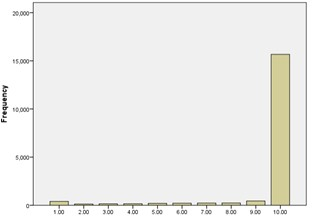
\includegraphics[scale=0.7]{dislgd1.jpg}
\caption{Distribution of LGDs between [0,1] }
\label{dis1}
\end{minipage}
\begin{minipage}[t]{0.5\linewidth}
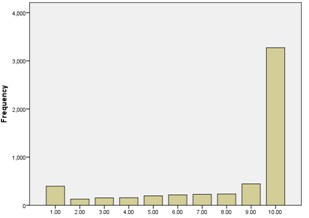
\includegraphics[scale=0.7]{dislgd2.jpg}
\caption{Distribution of LGDs between (0,1) }
\label{dis2}
\end{minipage}
\end{figure*}
\par
\vspace{-0.4in}
\hspace{-0.2in}

Through the preliminary analysis of the whole dataset, 35 variables and about 20000 accounts remains after screening. Meanwhile, LGD for online microloan shows a bimodal distribution is confirmed. Because so many accounts cannot repay back anything when default happen, so it is necessary to make a distinction between these accounts, which will be carefully explains in the next parts.

\subsection{Binary Models}
This part shows the result of Logistic regression model and Binary quantile regression model. Through comparing the KS index for both models, it is can be concluded that binary quantile regression is at least as good as Logistic regression model for the binary RR dataset. The following part is a detailed exposition of two models.

\subsubsection{Logistic Stepwise Regression Model \\} 
As mentioned before, we take logistic regression as our benchmark for binary quantile model, in which the KS is chosen as our statistical indicator to evaluate the 2 models and make comparison.\\
We use the stepwise option to choose significant regression variables.

\begin{table}[!h]
	\centering
	\caption{The Results of Logistic Regression} 
	\label{lres}
	\begin{tabular}{lrrrrr}
	\hline
	 Parameters &  \tabincell{r}{Degree of\\freedom} & Estimate & \tabincell{r}{Standard\\error}  & Wald & \tabincell{r}{Pr$>$Chi\\-square} \\ 
		\hline
		Intercept &   1 & -0.62 & 0.20 & 9.32 & 0.0023 \\ 
		ProsperRating &   1 & 0.08 & 0.03 & 8.74 & 0.0031 \\ 
		ListingCategory&   1 & 0.03 & 0.01 & 13.23 & 0.0003 \\ 
		TotalCreditLinespast7years &   1 & -0.01 & 0.00 & 14.67 & 0.0001 \\ 
		OpenRevolvingAccounts &   1 & 0.02 & 0.01 & 10.86 & 0.001 \\ 
		CurrentDelinquencies&   1 & 0.05 & 0.01 & 40.37 & $<$.0001 \\ 
		DelinquenciesLast7Years &   1 & -0.00 & 0.00 & 4.84 & 0.0277 \\ 
		BankcardUtilization &   1 & -0.19 & 0.07 & 7.94 & 0.0048 \\ 
		TradesNeverDelinquentpercent &   1 & 1.07 & 0.15 & 52.73 & $<$.0001 \\ 
		LoanOriginalAmount &   1 & -0.00 & 0.00 & 40.74 & $<$.0001 \\ 
		MonthlyLoanPayment &   1 & 0.00 & 0.00 & 48.48 & $<$.0001 \\ 
		Investors &   1 & -0.00 & 0.00 & 17.16 & $<$.0001 \\ 
		CreditHistory &   1 & -0.00 & 0.00 & 5.68 & 0.0171 \\ 
		clu\_ES\_1ind &   1 & -0.76 & 0.06 & 168.66 & $<$.0001 \\ 
		clu\_ES\_2ind &   1 & -0.27 & 0.06 & 21.24 & $<$.0001 \\ 
		CurrentlyInGroup\_Find &   1 & 0.47 & 0.05 & 74.27 & $<$.0001 \\ 
		IR\_1ind &   1 & 0.56 & 0.10 & 32.22 & $<$.0001 \\ 
		IR\_2ind &   1 & 0.61 & 0.10 & 37.84 & $<$.0001 \\ 
		IncomeVerifiable\_Find &   1 & 0.20 & 0.09 & 5.35 & 0.0208 \\ 
	\hline
	\end{tabular}
\end{table}

Table \ref{lres} is the maximum likelihood estimation analysis result in LR model. The last 6 variables stand for indicators of some class variables in \ref{intr1} named EmploymentStatus, CurrentlyInGroup, IncomeRange and IncomeVerifiable, the prefix 'clu' stans for clustered. We found these variables have a significant impact on RR after stepwise regression. There are some variables shows significant negative impact on $p_0$, so that a positive correlation with RR, these are bankcard utilization, employment status belong to full-time, part time, not available and not employed. It's easy to explain that borrowers who have bankcards obviously have higher credit.\\
Some of the rest of variables have negative correlation with RR and others show little impact. From literature part, a large number of studies have indicated that there was a relationship between PD and RR, current delinquencies is a kind of PD, result shows that current delinquencies take negative impact on RR. In another words, in the area of online microloan industry PD and RR exist negative correlation. From the coefficient of loan original amount, when the original amount bigger RR will be higher. 
However, from the result, the higher ProsperRating means the lower level of RR. We think it's because the high rating accounts make less default so that the default data set has screened more bad account of high rating.\\
For the online microloan market, persons' credit line, income range and credit history seems to be a kind of personal guarantee and income level as a personal security level. When a person has higher credit lines, higher income range and longer credit history, the RR will be higher.For the two groups of employment status, the result seems unusual, the person belongs to not employment and part-time have positive impact for RR. Conversely, the person belongs to self-employed, retire and others have negative impact on RR. The only explanation is that perhaps the population is unbalanced. \\
In general, the research on RR characteristics for online microloan and traditional bank exist in certain similarity, but related degree is not very high.

\subsubsection{Binary Quantile Model \\} 

The variables coefficient in binary quantile regression is estimated by R software. Totally there are 18 variables be test which is the same as Logistic regression model. Figure \ref{quant1} shows the coefficient for each variables in different quantile points. In the view of overall situation, most of the extreme values are generated in the head or tail, the middle part is relatively stable. It also indirectly shows the RR and LGD have a bimodal distribution characteristics. For some variables, although the size of the regression coefficient does not have a marginal impact, but the positive or negative sign can reflect the direction of the influence of the explanatory variables on the RR. Such as, employment status situation which indicates that the different employment status has different effects on RR and there was a significant heterogeneity at the high quantile points.\\
\par
\vspace{3in}
\hspace{3in}
\begin{figure}[!h]
		\quad\quad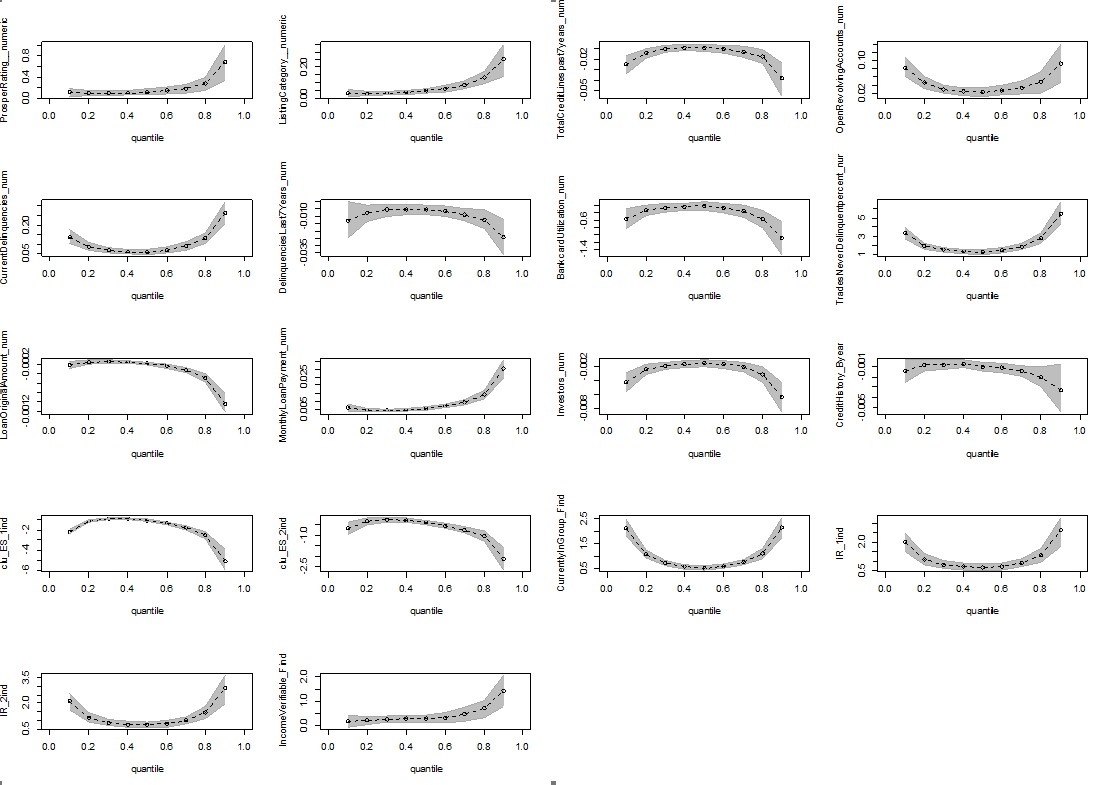
\includegraphics[height=0.06\textheight]{quant1.jpg}
	\caption{Quantile coefficient}
	\label{quant1}
\end{figure}

\begin{table}[!h]
\centering
	\caption{The Results of Quantile Regression} 
	\label{qres}
\begin{tabular}{lrrrrrrrrr}
  \hline
  Quantile & 0.1 & 0.2 & 0.3 & 0.4 & 0.5 & 0.6 & 0.7 & 0.8 & 0.9 \\ 
   \hline
  Intercept & -7.87 & -3.73 & -2.27 & -1.40 & -0.67 & -0.10 & 0.53 & 1.25 & 3.06 \\ 
  ProsperRating & 0.11 & 0.10 & 0.11 & 0.11 & 0.12 & 0.15 & 0.17 & 0.30 & 0.79 \\ 
  ListingCategory  & 0.03 & 0.03 & 0.03 & 0.04 & 0.05 & 0.06 & 0.09 & 0.14 & 0.27 \\ 
  TotalCreditLinespast7years  & -0.03 & -0.01 & -0.01 & -0.01 & -0.01 & -0.01 & -0.01 & -0.02 & -0.04 \\ 
  OpenRevolvingAccounts & 0.08 & 0.04 & 0.03 & 0.02 & 0.02 & 0.03 & 0.03 & 0.04 & 0.09 \\ 
  CurrentDelinquencies & 0.14 & 0.09 & 0.07 & 0.06 & 0.06 & 0.07 & 0.09 & 0.14 & 0.27 \\ 
  DelinquenciesLast7Years  & -0.02 & -0.01 & -0.01 & -0.01 & -0.01 & -0.01 & -0.01 & -0.01 & -0.02 \\ 
  BankcardUtilization & -0.58 & -0.33 & -0.27 & -0.22 & -0.21 & -0.28 & -0.33 & -0.58 & -1.04 \\ 
  TradesNeverDelinquentpercent  & 3.35 & 1.90 & 1.50 & 1.32 & 1.28 & 1.45 & 1.90 & 2.91 & 5.92 \\ 
  LoanOriginalAmount & -0.00 & -0.00 & -0.00 & -0.00 & -0.00 & -0.00 & -0.00 & -0.00 & -0.00 \\ 
  MonthlyLoanPayment & 0.01 & 0.00 & 0.00 & 0.00 & 0.01 & 0.01 & 0.01 & 0.02 & 0.03 \\ 
  Investors & -0.00 & -0.00 & -0.00 & -0.00 & -0.00 & -0.00 & -0.00 & -0.00 & -0.01 \\ 
  CreditHistory  & -0.00 & -0.00 & -0.00 & -0.00 & -0.00 & -0.00 & -0.00 & -0.00 & -0.00 \\ 
  clu\_ES\_1ind & -2.13 & -1.15 & -0.88 & -0.88 & -1.04 & -1.36 & -1.82 & -2.63 & -5.53 \\ 
  clu\_ES\_2ind & -0.70 & -0.34 & -0.27 & -0.29 & -0.39 & -0.55 & -0.75 & -1.09 & -2.30 \\ 
  CurrentlyInGroup\_Find & 2.15 & 1.10 & 0.74 & 0.57 & 0.52 & 0.60 & 0.76 & 1.12 & 2.16 \\ 
  IR\_1ind & 1.98 & 1.11 & 0.83 & 0.72 & 0.70 & 0.76 & 0.93 & 1.38 & 2.92 \\ 
  IR\_2ind & 2.10 & 1.20 & 0.88 & 0.78 & 0.75 & 0.83 & 1.02 & 1.51 & 3.15 \\ 
  IncomeVerifiable\_Find & 0.21 & 0.20 & 0.27 & 0.30 & 0.30 & 0.36 & 0.41 & 0.75 & 1.55 \\ 
   \hline
\end{tabular}
\end{table}


The coefficients have changed a little in binary quantile regression if compare to logistic regression. In these parameters, the intercept cross the range from negative to positive. Some variables coefficients fall completely in the negative range, which are TotalCreditLinespast7years, DelinquenciesLast7Years, BankcardUtilization, clu\_ES\_1ind and clu\_ES\_1ind. In the whole of quantile, these variables take negative impact to $p_0$ so positive impact to RR. These results is in accordance with those in logistic regression. The rest of the variables have a more or less positive effect on RR. In a word, binary quantile regression model agree with logistic regression model mostly.


\subsubsection{ Comparison results\\} 
Above is the result of parameters from the process of training sample. In order to compare the accuracy and degree of fitting between two models, validation set variables will be brought into the models and obtain the prediction value of RR, then compare to the real RR. Table \ref{lks} and Table \ref{qks} shows two models Kolmogorov-Smirnov Two-sample test result respectively.

\begin{table}[!h]
\centering
	\caption{Logistic regression KS test} 
	\label{lks}
\begin{tabular}{|l|r|l|r|}
  \hline
 \multicolumn{4}{|c|}{Kolmogorov Smirnov Two sample test }\\ 
  \hline
  KS & 0.13 & D & 0.279457 \\ 
	\hline
  KSa & 8.94 & Pr $>$ KSa & $<$.0001 \\ 
	\hline
  CM & 0.01 & CMa & 40.975078 \\ 
   \hline
\end{tabular}
\end{table}
\vspace{-0.2in}

\begin{table}[!h]
\centering
	\caption{Quantile regression KS test} 
	\label{qks}
\begin{tabular}{|l|r|l|r|}
  \hline
 \multicolumn{4}{|c|}{Kolmogorov Smirnov Two sample test }\\ 
  \hline
  KS & 0.12 & D & 0.254130  \\ 
	\hline
  KSa & 8.13 & Pr $>$ KSa & $<$.0001 \\ 
	\hline
  CM & 0.01 & CMa & 40.432716 \\ 
   \hline
\end{tabular}
\end{table}

Comparing the KS value in the two tables, Binary quantile regression model hold similar KS value to Logistic regression model, this means relative ability to distinguish zeros and non-zeros values of RR. Meanwhile, the p-value of KS also proves the predicted probability distribution is significantly different under 2 classes, which means the ability of distinguishing to be strong. With the above analysis, for the binary RR data set, Binary quantile regression model can make accurate predictions as well as logistic regression model. Especially to deserve to be mentioned, the binary quantile regression model is more promising because more quantiles can be added so that the result will be improved then.

\subsection{Linear Regression and Quantile Regression}
In this section, we'll test RR that falls in the range of 0 to 1, totally 3848 observations. For the missing data, the repair method is consistent with the previous. The split of the training set and the validation set is still in a random way. Four types of data transformation be used for the processing of RR, for the different transformation, SAS system through backward test automatically match the best variables then get the regressive equation. Root mean square error (RMSE) as the evaluation index, the best data transformation results be used for quantile regression. 

\subsubsection{General Linear Regression Model \\} 
Following are the RR distribution and four transformation results.\\
\par
\vspace{0.7in}
\hspace{0.7in}
\begin{figure*}[!h]
		\quad\quad\quad\quad\quad\quad\quad\quad\quad\quad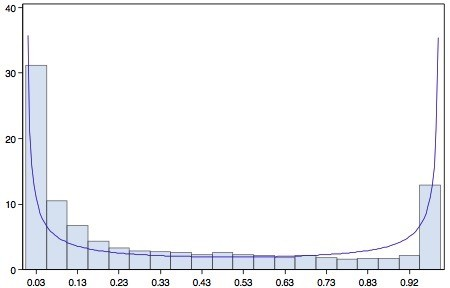
\includegraphics[scale=0.7]{rrdis.jpg}
	\caption{RR distribution under Beta transformation}
	\label{rrdis}
\end{figure*}
\par
\vspace{-0.3in}

\begin{table}[!h]
\centering
	\caption{ Fractional logit transformation result} 
	\label{ftrs}
\begin{tabular}{lrr}
	\hline
		Parameter&	Estimate	& Pr$>$\mid t\mid\\
		\hline
		Intercept&	3.704 &	$<$.0001\\
		IR\_1	&1.442& 	$<$.0001\\
		IR\_2	&1.055 &	0.0009\\
		IncomeVerifiable\_False&	-0.687 	&0.1081\\
		ProsperRating	&-0.435 	&0.0014\\
		ListingCategory	&-0.077 	&0.0517\\
		OpenRevolvingMonthlyPayment	&0.001 	&0.0004\\
		InquiriesLast6Months	&-0.065 	&0.0123\\
		CurrentDelinquencies	&-0.101 	&0.0036\\
		RevolvingCreditBalance	&0.000 	&0.0183\\
		TradesNeverDelinquentpercent	&-2.271 &	0.0004\\
		DebtToIncomeRatio	&0.225 	&0.1441\\
		LoanOriginalAmount	&0.001 &	$<$.0001\\
		MonthlyLoanPayment &	-0.039& 	$<$.0001\\
		InvestmentFromFriendsCount	&-0.969 &	0.0256\\
		InvestmentFromFriendsAmount	&0.000 	&0.1425\\
  \hline
\end{tabular}
\end{table}

\begin{table}[!h]
\centering
	\caption{Log-log transformation result} 
	\label{lltrs}
\begin{tabular}{lrr}
\hline
	Parameter&	Estimate	& Pr$>$\mid t\mid\\
	\hline
	Intercept	&5.037 	&$<$.0001\\
	IR\_1	&0.707 &	0.0079\\
	IR\_2	&0.389 &	0.1522\\
	IncomeVerifiable\_False	&-0.652 	&0.0752\\
	ProsperRating	&-0.355 &	0.0024\\
	ListingCategory	&-0.081 	&0.0183\\
	OpenRevolvingMonthlyPayment&	0.001 	&0.0031\\
	TotalInquiries	&-0.017 &	0.0327\\
	CurrentDelinquencies	&-0.069 	&0.0199\\
	RevolvingCreditBalance	&0.000 &	0.0602\\
	TradesNeverDelinquentpercent	&-2.092 	&0.0001\\
	DebtToIncomeRatio	&0.238 	&0.0719\\
	LoanOriginalAmount	&0.001 	&$<$.0001\\
	MonthlyLoanPayment	&-0.036 	&$<$.0001\\
	InvestmentFromFriendsCount	&-0.549 &	0.1001\\
	\hline
\end{tabular}
\end{table}

\begin{table}[!h]
\centering
	\caption{Beta transformation result} 
	\label{btrs}
\begin{tabular}{lrr}
  \hline
	Parameter&	Estimate	& Pr$>$\mid t\mid\\
	\hline
	Intercept&	0.409 	&0.0008\\
	IR\_1	&0.279 &	$<$.0001\\
	IR\_2	&0.212 	&$<$.0001\\
	ProsperRating	&-0.066 	&0.003\\
	ListingCategory	&-0.013 &	0.0503\\
	OpenRevolvingMonthlyPayment	&0.000 	&0.0009\\
	InquiriesLast6Months&	-0.012 &	0.0055\\
	CurrentDelinquencies	&-0.018 &	0.0018\\
	RevolvingCreditBalance	&0.000 	&0.0073\\
	TotalTrades	&0.002 	&0.1561\\
	TradesNeverDelinquentpercent	&-0.360 	&0.0007\\
	LoanOriginalAmount	&0.000 &	$<$.0001\\
	MonthlyLoanPayment	&-0.006 	&$<$.0001\\
	InvestmentFromFriendsCount	&-0.162 	&0.0235\\
	InvestmentFromFriendsAmount&	0.000 &	0.145\\
	\hline
\end{tabular}
\end{table}

\begin{table}[!h]
\centering
	\caption{Probit transformation result} 
	\label{ptrs}
\begin{tabular}{lrr}
  \hline
	Parameter&	Estimate	& Pr$>$\mid t\mid\\
	\hline
	Intercept&	0.213 	&0.0761\\
	CurrentlyInGroup\_False&	0.067 	&0.0951\\
	IR\_1&	0.392 	&$<$.0001\\
	IR\_2	&0.325 &	$<$.0001\\
	ProsperRating	&-0.058 	&0.0089\\
	OpenRevolvingMonthlyPayment&	0.000 &	$<$.0001\\
	InquiriesLast6Months	&-0.012 &	0.0051\\
	CurrentDelinquencies	&-0.018 	&0.0012\\
	RevolvingCreditBalance	&0.000 	&0.0008\\
	TotalTrades	&0.002 	&0.1171\\
	TradesNeverDelinquentpercent	&-0.273 &	0.0088\\
	LoanOriginalAmount	&0.000 &	$<$.0001\\
	MonthlyLoanPayment	&-0.004 &	$<$.0001\\
	Recommendations	&-0.076 	&0.038\\
	InvestmentFromFriendsAmount	&0.000 	&0.1123\\
	Investors	&0.000 &	0.0544\\
	\hline
\end{tabular}
\end{table}

Observing the above results, although each transformation has a slightly different in variable selection, the core variables are nearly the same if compared with the logistic regression. Such as income range, revolving credit balance, loan original amount and monthly loan payment etc. In other words, the influence factors of RR or LGD have a certain relationship with the traditional banks. After regression simulation for the validation set, from RMSE results in Table \ref{rmse}, beta transformation and probit transformation has a better degree of fitting if compare with others. Since probit transformation has some difficulties in the quantile model applications, beta transformation will be chosen to apply to quantile model. Another reason to select beta transformation is RR presents a clear bimodal structure when beta be used, Figure \ref{rrdis} shows RR distribution under Beta transformation and give us a very intuitive bimodal structure feeling. This obeyed the LGD structure which has been mentioned in the literature review part and indirectly indicate the reliability of beta transformation.

\begin{table}[!h]
\centering
	\caption{Four types transformation RMSE result} 
	\label{rmse}
\begin{tabular}{|l|c|c|c|c|}
  \hline
Transformations	&Fractional logit	&Log-log	&Beta	&Probit\\
\hline
RMSE	&0.7225&	0.7394	&0.6126&	0.4220\\
   \hline
\end{tabular}
\end{table}

\subsubsection{Beta-Trans Quantile Model \\} 
Using the beta transformation of RR, we analyze them in different quantiles to build the quantile regression model. Figure \ref{qbtrs} shows coefficients and the confidences of different variables from quantile 0.1 to 0.9.

\begin{figure*}[!h]
\vspace{1.5in}
\begin{minipage}[t]{0.5\linewidth}
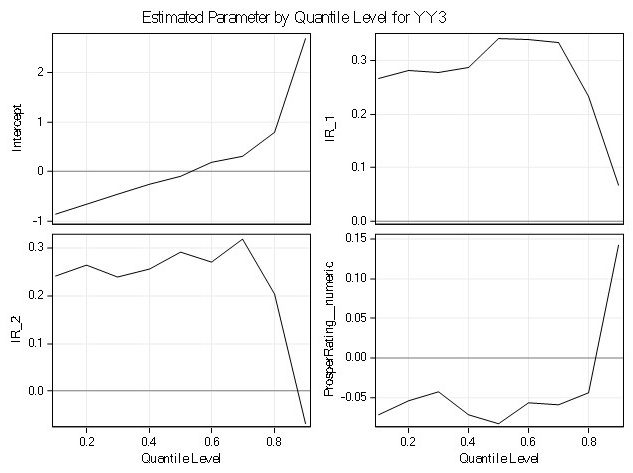
\includegraphics[scale=0.4]{beta1.jpg}
\end{minipage}
\begin{minipage}[t]{0.5\linewidth}
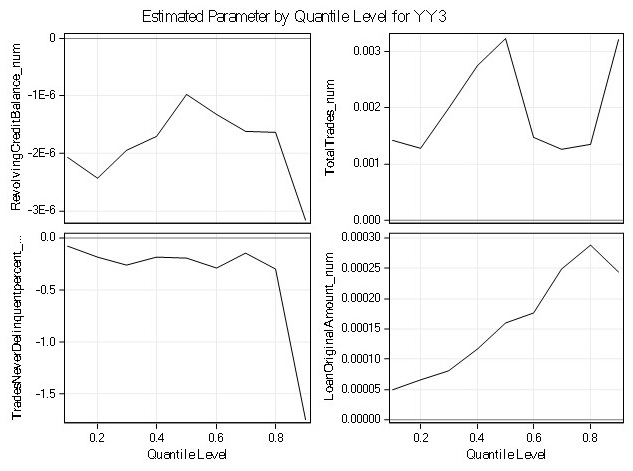
\includegraphics[scale=0.4]{beta2.jpg}\\
\end{minipage}
\par
\vspace{1.5in}
\begin{minipage}[t]{0.5\linewidth}
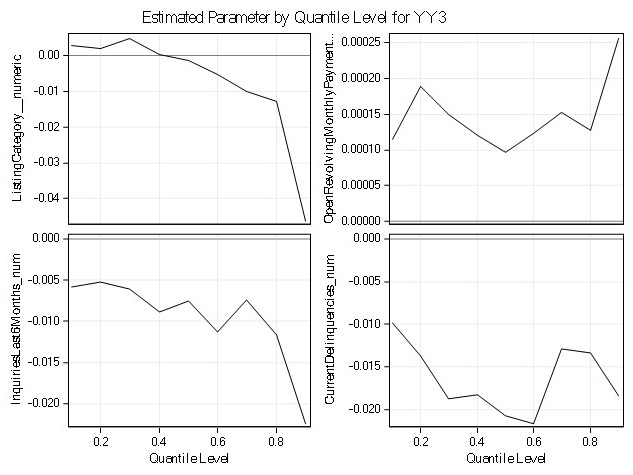
\includegraphics[scale=0.4]{beta3.jpg}
\end{minipage}
\begin{minipage}[t]{0.5\linewidth}
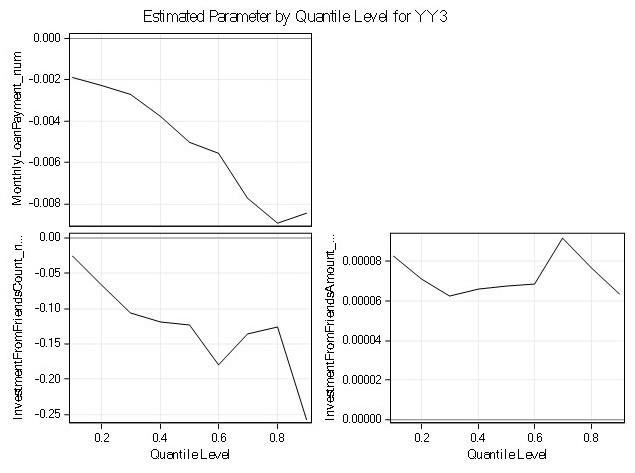
\includegraphics[scale=0.4]{beta4.jpg}
\end{minipage}
\caption{Estimated parameter by quantile level for Beta transformation}
\label{qbtrs}
\end{figure*}
Comparing with binary RR quantile result, at this time the coefficients of each variables has a huge wave, it is clear observation of the change in each quantile. In general, most of the extreme values are generated in the tail, which is because RR presents a special extreme value distribution. For more details, in most instances, income range have positive relationship with RR, but when RR fall in the last 30\% of the interval, the impact will be significantly decreased and close to 0. For the Prosper rating, listing category, inquiries last 6 months and trades never delinquent percent, in the first 80\% intervals, their impact is very smooth, but there is a great change in the last 20\% intervals. Monthly loan payment and investment from friends count has negative impact for RR and the impact will be stronger when RR increase. The methods of multiple analytical in various range make quantile regression has stronger analytical skills and each interval has its own characteristics. Table \ref{qrmse} shows the result of RMSE for linear regression under beta transformation and probit transformation and quantile regression model, after the observation of the validation set, quantile regression shows the best degree of fitting in the three, which illustrates \citet{Somers2007} viewpoint that quantile regression might be helpful to solve some problems when the distribution is highly non-normal.

\begin{table}[!h]
\centering
	\caption{Beta/Probit transformation and Quantile regression RMSE result} 
	\label{qrmse}
\begin{tabular}{|l|c|c|c|}
  \hline
Models	&Beta transformation	&Probit transformation&	Quantile regression\\
\hline
RMSE	&0.6126	&0.4220	&0.3437\\
   \hline
\end{tabular}
\end{table}

\section{Summary and Prospected}\label{sec:conclusion}
\subsection{Summary}

Based on the theoretical analysis of the effects of various factors on the heterogeneity of RR, using different models as benchmarks, we make analysis of the degree of fitting of RR focused on the quantile regression model. On one hand, through analyzing the size and sign of the quantile regression coefficient, the heterogeneity of impact was revealed. On the other hand, through comparing the evaluation indicators KS and RMSE, observation prediction results and degree of fitting was shown clearly. The empirical results shows that quantile regression model has obvious advantages.\\
Firstly, in general speaking, the LGD distribution on online microloan has a bimodal distribution. There is a certain similarity with the traditional banking, the difference is that the LGD in online microloan have a very high peak in the tail, which means when an account default the totally loss cannot be recover in most cases. The online microloans risk is much higher than the traditional banking. Secondly, for the binary RR data set, logistic regression and binary quantile regression be compared. By observing the evaluation indicators KS, the accuracy of binary quantile regression is at least as good as logistic regression. From the coefficient estimation, the extreme value mostly appear in the header and trailer, the middle part is relatively stable. For the online microloan companies, monitor and tracking these accounts in that ranges can reduce the loss.
Thirdly, for the RR falls in the interval 0 to 1, linear regression with four types of variables transformation and quantile regression was compared. By observing the evaluation indicators RMSE, we found that quantile regression model shows higher accuracy than linear regression model. From the observation of coefficient estimation, there is a huge mutation in the tails. There is a similarity with the previous results.\\
Can foreknow, due to the heterogeneity of online microloan behavior, quantile regression model will play a more and more important role in the research of risk, it has confirmed \citet{Somers2007}.\\
Remarks: when the distribution was highly non-normal and understanding the changes in the dispersion around the mean was helpful, resulted that forecasting distribution using quantile regression would made a difference, at the same time, quantile regression would provide more comprehensive descriptions of the data than regressions for the mean response.

\subsection{Prospected}

Compared with the classical least square regression, quantile regression is a new and comprehensive statistical method. It can measure the direct relationship between the variables and the regression variables in different quantile, so it has a unique advantage in the application. Quantile regression has only a short history about twenty to thirty years, so a lot of theoretical problems and statistical methods are needed to be further studied. Such as quantile regression time series, number of goodness of fit test and Bayesian quantile regression, they not only well solves the existing quantile regression of some of the problems, but also got the greater attention to this model.\\
The rapid development of the Internet platform create a good opportunity to online microloan. In order to take more benefits and efficiently on both side of company and customer. On the basis of reasonable operation, they must have a complete set of internal risk analysis system and risk management experience. In order to realize this goal, the combination of the model and the actual situation is particularly important.
In short, in the area of quantile regression theory and P2P online microloans platform, we still need to continue to learn, continue to explore and explain the new problems, to solve the new difficulties, to make us continue to move forward.\\

\section{Acknowledgement:}

%\section{Appendix: Regression Spline Function}\label{sec:Splines}

\bibliographystyle{ormsv080}
\newpage
\bibliography{CM1129}

\end{document}


